%\scalebox{0.8}{\textit{Reference: Gaddis Chapter 4}}

Repetition structures (loops) are one of the best justifications for moving from Excel to Python (though they are not unique to Python). A ``program''
in Excel is a serious of keystrokes and clicks. You might create a report for your company that is specific to one
market and you'll need to replicate the same report for a different market. Perhaps you could write a macro, but
I think you'll find working in Python to be easier. In Python, we can do this in a loop. We can have a program that makes the report and we
can iterate through the different markets to apply the program to each and create the specific reports (using a for loop).

We also introduce the idea of an \emph{iterable} object. 


\section{While Loops}
 
The \textbf{while loop} is a condition-controlled loop. Figure \ref{fig:while} illustrates the logic well.

%% Figure
\begin{figure}[h!] 
\begin{center} 
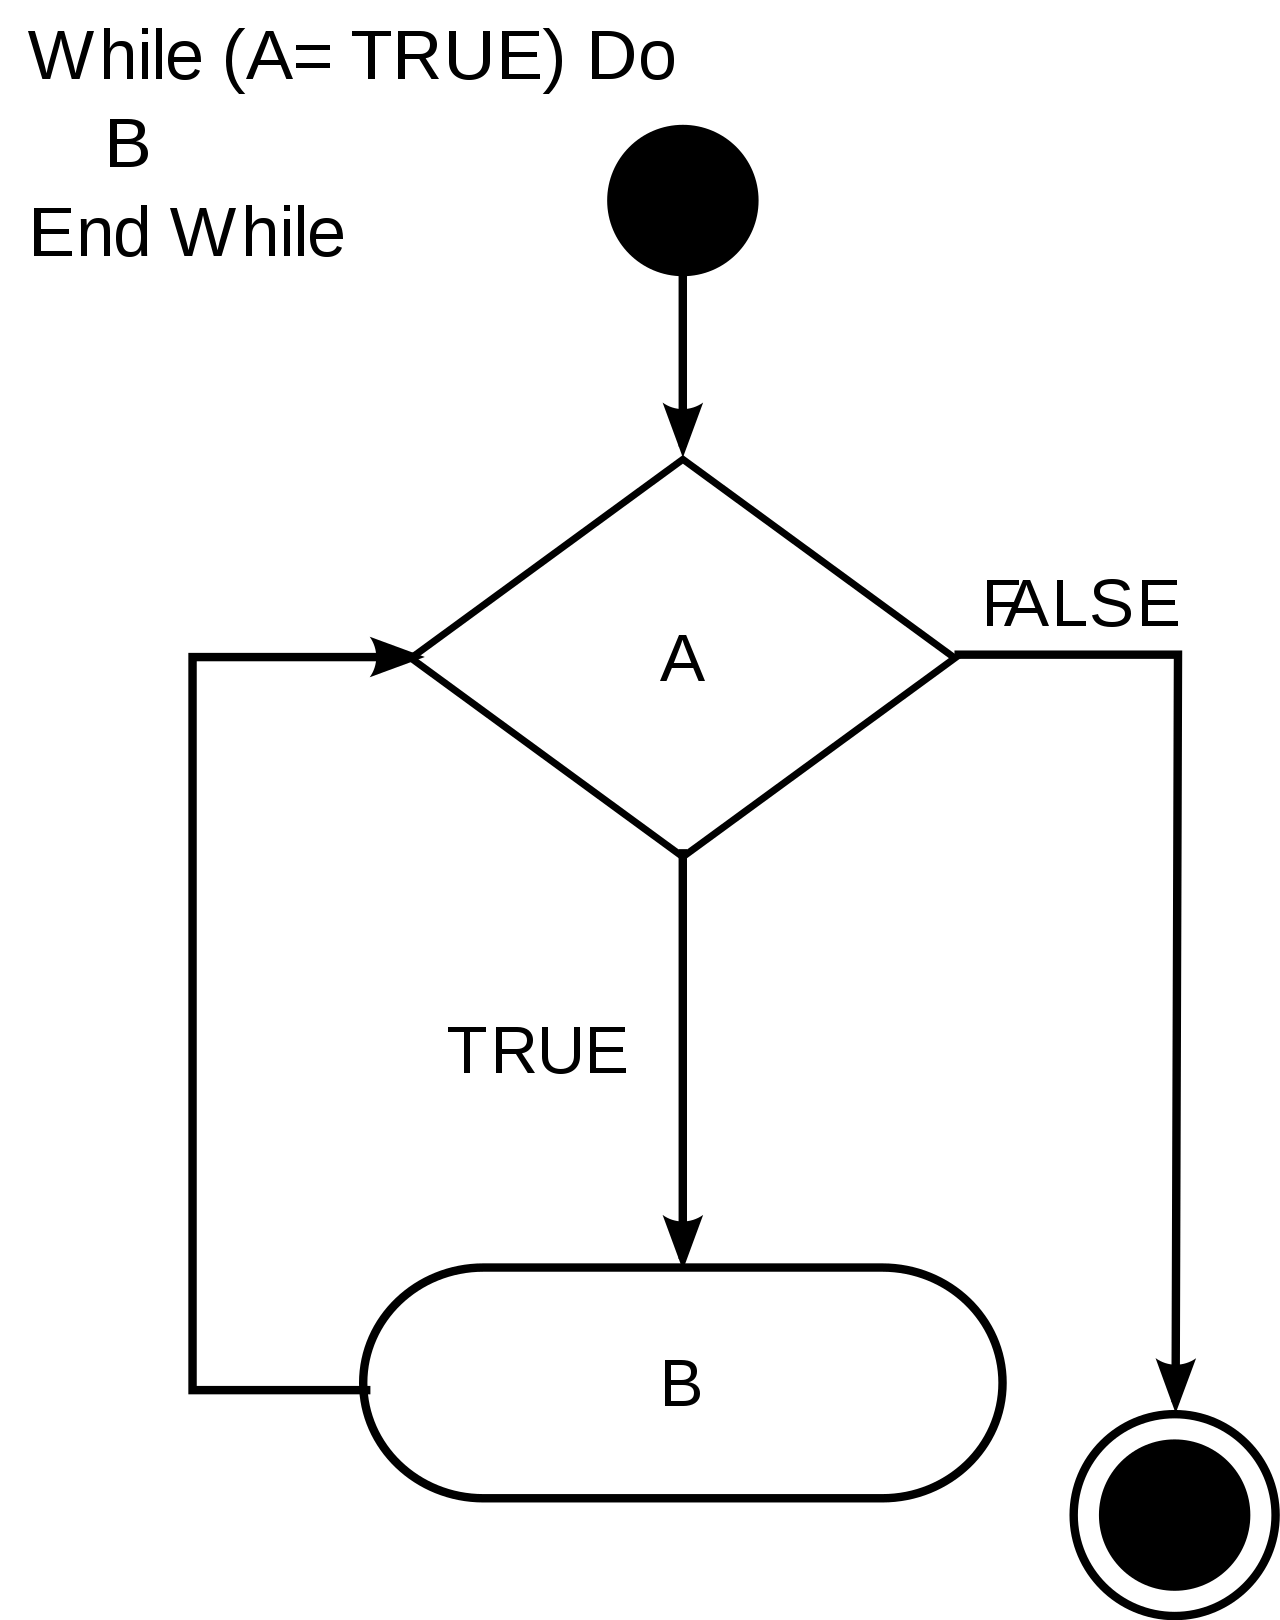
\includegraphics[width = .55\textwidth]{while_loop.png}
\caption{While loop logic (\textcolor{blue}{\href{https://en.wikipedia.org/wiki/While\_loop}{Wikipedia}}).}
\label{fig:while}
\end{center}
\end{figure}


\smallskip

\noindent The statement inside a while loop executes as long as the condition evaluates to True.

\begin{lstlisting}[language = Python]
# Rest on the seventh day
day_of_week = 1
while day_of_week < 7:
    print('work')
    day_of_week += 1 \end{lstlisting}


\smallskip
\noindent Beware the infinite loop. Be confident that your test condition will have a way of becoming False, otherwise
you might notice that your program never finishes. 

\smallskip

\noindent Let's consider an infinite series, $\sum_{i=0}^\infty 2^{-i} =  1 + \frac{1}{2} + \frac{1}{4} + \frac{1}{8} + \dots = 2$.
We could try to calculate this with a while loop if we didn't know the sum converged to two.

\begin{lstlisting}[language = Python]
# Sum of a geometric series
the_sum = 0
idx = 0
increment = 2 ** -idx

while increment > 0:
    # Increase the sum by the current increment
    the_sum += increment
    
    # Advance the index in the sum and calculate a new increment
    idx += 1
    increment = 2 ** (-idx) \end{lstlisting}
    
\smallskip

\noindent Does this loop make you nervous? In fact, the loop will terminate because we will eventually hit machine zero.
I found the loop to terminate at the increment $2^{-1075}$ and the resulting sum to be two. But it should make you nervous.
You might instead decide on some level of precision and use a test condition like 
\lstinline[language=Python]{increment > .0005}, in which case you could find a bound on the error with some math.
Doing that math is not part of this course, (un)fortunately.


\section{For Loops} 
\label{sec:forloop}

For loops execute the attached code based on some iteration. The code might depend on a variable that is actually changing
with the iteration. 

\begin{lstlisting}
#Dr. Seuss
for item in [1,2,'red','blue']:
    print(item, 'fish')  
\end{lstlisting}

The general structure is 
% random Pascal language to avoid highlighting
\begin{lstlisting}[language = Pascal] 
for <iteration_variable> in <iterable>:
    <program>
\end{lstlisting}
The iteration variable should be chosen to maximize readability. 

Sometimes you find definitions for \textbf{iterable} that are circular, like ``objects that can be iterated over.'' It's something where we can traverse through distinct values. So far, the iterables we have seen are strings and lists. A for loop will iterate over a list one element at a time, according to the ordering in the list. A for loop iterates over a string one character at a time. There are several more types of iterable objects, but for now the only additional one we'll introduce is that created by \code{range(start, stop, step)}, which allows you to iterate over integers from \code{start} (inclusive) to \code{stop} (exclusive) according to the \code{step} parameter. By default, \code{start = 0} and \code{step = 1} so these are optional arguments. You can check what is included in a particular call to \code{range()} by examining \code{list(range(start, stop, step))}.

\smallskip

\noindent The for clause tells Python to execute the statement once for every item in the iterable, which is
in this case the object \code{[1,2,'red','blue']}. This is a \emph{list}, a kind of 
compound data object that can store other objects in sequence by separating them with commas and putting
them inside square brackets. Below we use \code{range(5)} instead of a list, which you
can think of as generating an iterable object of integers from 0 to 4 (5 is not included, but the length is 5).


\smallskip

\noindent Or you might just want to execute a specific set of statements some number of times.


\begin{lstlisting}[language = Python]
# Tubthumping by Chumbawamba
for item in range(5):
    print("I get knocked down, but I get up again.")
    print("You are never gonna keep me down.") \end{lstlisting}

\smallskip

\noindent For both of the examples above, \lstinline[language = Python]{item} is the \emph{variable}. However, notice
the print statement only depends on the variable in the first example.

\smallskip
\noindent You can even iterate over the characters in a string.

\begin{lstlisting}[language = Python]
# Cheer
word = 'PYTHON'
for char in word:
    print("Give me a",char, '!')
    print("    ", char)
print("What's that spell?")
print("    ",word) \end{lstlisting}


\subsection{Nested Loops}

A loop that is inside another is called \emph{nested}.

\smallskip
\noindent Think about how Python executes code line by line. What order of output do you expect from this program?


\begin{lstlisting}[language = Python]
# Nested Loop
for x in ['wee', 'bee']:
    for y in ['bop', 'dop']:
        print(x,y) \end{lstlisting}

If it helps, the above is a simplification of the following. 


\begin{lstlisting}
# Nested Loop
x = 'wee'
for y in ['bop', 'dop']:
    print(x,y) 

x = 'bee'
for y in ['bop', 'dop']:
    print(x,y)   
\end{lstlisting}



\smallskip
